\documentclass[11pt]{article}

\usepackage[utf8]{inputenc}
\usepackage[T1]{fontenc}
\usepackage{lmodern}
\usepackage{geometry}
\geometry{margin=1in}
\usepackage{amsmath,amssymb,amsfonts,amsthm,mathtools,bm}
\usepackage{physics}
\usepackage{tikz}
\usetikzlibrary{arrows.meta,positioning,calc,decorations.pathmorphing,patterns,shapes.geometric}
\usepackage{hyperref}
\usepackage{enumitem}
\usepackage{authblk}

\hypersetup{colorlinks=true,linkcolor=blue,citecolor=blue,urlcolor=blue}

\newtheorem{theorem}{Theorem}
\newtheorem{proposition}{Proposition}
\newtheorem{lemma}{Lemma}
\newtheorem{definition}{Definition}
\newtheorem{corollary}{Corollary}
\theoremstyle{remark}
\newtheorem{remark}{Remark}

\title{What Lattice QCD Can and Cannot Simulate About Gravity: A Fixed-Background Theorem and Computational Roadmap}
\author{Author Name}
\affil{Independent Research Draft}
\date{Draft \today}

\begin{document}
\maketitle

\begin{abstract}
Modern lattice QCD uses leadership-class and exascale computing to evaluate nonperturbative quark and gluon dynamics. This has motivated the question of whether the same computational machinery can simulate gravitons or the emergence of gravity from quantum fields. This paper introduces a precise separation between three computational layers: lattice QCD on a fixed background, lattice field theory on prescribed curved spacetime, and lattice quantum gravity with dynamical geometry. The central theorem states that a fixed-background lattice QCD path integral can compute matter correlators and stress-energy response to a prescribed metric, but cannot by itself generate a graviton propagator or dynamical spacetime degrees of freedom because the metric is not integrated over. A constructive roadmap is then proposed: use lattice gauge theory to compute $\langle T_{\mu\nu}\rangle$ and equation-of-state data, feed these into semiclassical gravity solvers, and reserve true graviton/emergent-geometry questions for dynamical lattice gravity frameworks such as causal dynamical triangulations or other nonperturbative quantum-gravity approaches.
\end{abstract}

\tableofcontents

\section{Introduction}

Lattice QCD (LQCD) is one of the most successful nonperturbative computational methods in physics. It discretizes spacetime, samples gauge-field configurations, and extracts hadronic observables from Euclidean correlation functions. Because gravitons are also quantum excitations of a field---the metric perturbation in weak-field quantum gravity---one may ask whether sufficiently powerful LQCD supercomputers can simulate gravitons directly.

This paper argues that the answer is structurally no, not merely computationally no. Standard LQCD holds the background geometry fixed. A graviton requires metric fluctuations or a dynamical geometry. Therefore, a bigger QCD lattice is not automatically a quantum-gravity simulator.

\paragraph{New viewpoint.} The paper frames the issue as a hierarchy of path integrals. The question is not ``Are supercomputers strong enough?'' but ``Which degrees of freedom are included in the measure?''

\section{Literature grounding}

Standard LQCD discretizes Euclidean spacetime, placing quark fields on sites and gauge links on edges. Extensions can place quantum fields on a prescribed curved classical background. Separately, nonperturbative quantum-gravity programs such as causal dynamical triangulations (CDT), Euclidean dynamical triangulations, spin foams, Regge calculus, and asymptotic-safety-inspired lattice studies attempt to sum over geometry itself. CDT in particular constructs a gravitational path integral from causal triangulated spacetimes, with dynamical adjacency relations and geometry.

\section{Three computational layers}

\begin{definition}[Fixed-background lattice QCD]
A fixed-background lattice QCD system is a path integral of the form
\begin{equation}
Z_{\rm QCD}[g]=\int \mathcal D U\,\mathcal D\bar\psi\,\mathcal D\psi\;e^{-S_{\rm QCD}[U,\bar\psi,\psi;g]},
\end{equation}
where $g$ is a prescribed background metric or, in standard simulations, a fixed Euclidean lattice geometry.
\end{definition}

\begin{definition}[Matter on curved background]
A matter-on-curved-background calculation permits $g_{\mu\nu}(x)$ to be nontrivial but fixed. One may compute
\begin{equation}
\langle T_{\mu\nu}(x)\rangle_g=\frac{2}{\sqrt g}\frac{\delta \ln Z_{\rm matter}[g]}{\delta g^{\mu\nu}(x)}.
\end{equation}
\end{definition}

\begin{definition}[Dynamical lattice gravity]
A dynamical lattice gravity path integral sums or integrates over geometric degrees of freedom:
\begin{equation}
Z_{\rm grav}=\sum_{\mathcal T}\frac{1}{C_{\mathcal T}}\int \mathcal D \ell\;e^{-S_{\rm grav}[\mathcal T,\ell]}Z_{\rm matter}[\mathcal T,\ell],
\end{equation}
where $\mathcal T$ denotes triangulations, connectivity, or discrete geometries, and $\ell$ denotes edge lengths or related metric data.
\end{definition}

\begin{figure}[h]
\centering
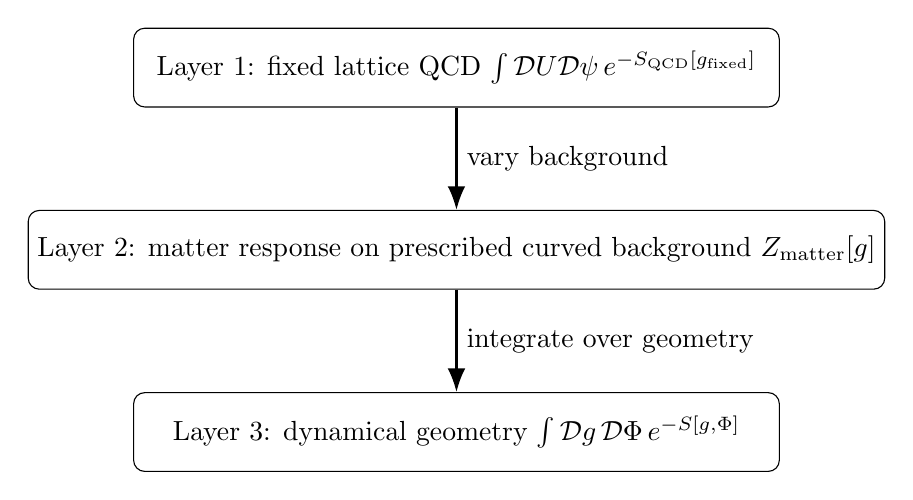
\begin{tikzpicture}[node distance=1.3cm]
    \node[draw,rounded corners,minimum width=8.2cm,minimum height=1cm] (a) {Layer 1: fixed lattice QCD $\int \mathcal DU\mathcal D\psi\,e^{-S_{\rm QCD}[g_{\rm fixed}]}$};
    \node[draw,rounded corners,minimum width=8.2cm,minimum height=1cm,below=of a] (b) {Layer 2: matter response on prescribed curved background $Z_{\rm matter}[g]$};
    \node[draw,rounded corners,minimum width=8.2cm,minimum height=1cm,below=of b] (c) {Layer 3: dynamical geometry $\int \mathcal Dg\,\mathcal D\Phi\,e^{-S[g,\Phi]}$};
    \draw[-{Latex[length=3mm]},thick] (a) -- (b) node[midway,right] {vary background};
    \draw[-{Latex[length=3mm]},thick] (b) -- (c) node[midway,right] {integrate over geometry};
\end{tikzpicture}
\caption{The crucial transition is not lattice size but whether geometry is included in the path-integral measure.}
\end{figure}

\section{Fixed-background theorem}

\begin{theorem}[No dynamical graviton from fixed-background LQCD]
Let
\begin{equation}
Z[g]=\int \mathcal D\Phi\;e^{-S[\Phi;g]}
\end{equation}
be a quantum field theory path integral over matter/gauge fields $\Phi$ with a prescribed, non-integrated metric $g$. Then $Z[g]$ can generate matter correlators and metric-response functions such as $\langle T_{\mu\nu}\rangle_g$, but it cannot produce a dynamical graviton propagator as an internal quantum correlator unless the metric or metric perturbation is itself included among the integrated fields.
\end{theorem}

\begin{proof}
Correlation functions generated by $Z[g]$ are obtained by differentiating with respect to sources coupled to fields integrated in the measure, or by differentiating with respect to external parameters such as $g$. Since $g$ is not integrated over, it has no quantum fluctuations in this path integral. Functional derivatives with respect to $g$ generate stress-energy insertions,
\begin{equation}
\frac{\delta \ln Z[g]}{\delta g^{\mu\nu}}\sim \langle T_{\mu\nu}\rangle_g,
\end{equation}
and higher derivatives generate stress-energy response functions. They do not generate a metric two-point function
\begin{equation}
\langle h_{\mu\nu}(x)h_{\rho\sigma}(y)\rangle
\end{equation}
unless $h_{\mu\nu}$ is itself a quantum variable in the path integral. Therefore, fixed-background LQCD cannot by itself simulate a dynamical graviton.
\end{proof}

\begin{corollary}[Supercomputer scaling is not enough]
Increasing lattice volume, decreasing lattice spacing, or improving Monte Carlo statistics does not change the field content of the path integral. A fixed-background simulation remains fixed-background regardless of computational scale.
\end{corollary}


\subsection{Metric-response hierarchy from the generating functional}
The fixed-background formalism contains more gravitational information than the one-point function alone. Define the Euclidean effective action
\begin{equation}
 W[g]\equiv-\ln Z[g].
\end{equation}
With the convention
\begin{equation}
 \langle T_{\mu\nu}(x)\rangle_g
 =\frac{2}{\sqrt{g(x)}}\frac{\delta W}{\delta g^{\mu\nu}(x)},
 \label{eq:lqcd-onepoint}
\end{equation}
the second metric derivative defines the matter polarization kernel
\begin{equation}
 \Pi_{\mu\nu,\rho\sigma}(x,y)
 \equiv
 \frac{4}{\sqrt{g(x)}\sqrt{g(y)}}
 \frac{\delta^2W}
 {\delta g^{\mu\nu}(x)\delta g^{\rho\sigma}(y)}.
 \label{eq:lqcd-polarization}
\end{equation}
Up to the contact terms generated by varying the stress tensor itself, $\Pi$ is the connected $TT$ correlator. A small external metric perturbation obeys the linear-response relation
\begin{equation}
 \delta\langle T_{\mu\nu}(x)\rangle
 =\frac12\int d^4y\sqrt{g(y)}\,
 \Pi_{\mu\nu,\rho\sigma}(x,y)h^{\rho\sigma}(y)
 +O(h^2).
 \label{eq:lqcd-linear-response}
\end{equation}

\begin{proposition}[Matter-dressed metric response]
Suppose an independent gravitational action supplies a linearized Einstein operator $\mathcal E$ about a background $\bar g$. Then the semiclassical perturbation equation can be written schematically as
\begin{equation}
 \left(\mathcal E-4\pi G\,\Pi\right)h
 =8\pi G\,\delta T_{\rm ext}.
 \label{eq:dressed-gravity-response}
\end{equation}
Consequently, fixed-background lattice data can determine the matter dressing $\Pi$ of a gravitational propagator even though the lattice matter path integral does not itself supply the bare metric kinetic operator $\mathcal E$.
\end{proposition}

\begin{proof}
Linearizing $G_{\mu\nu}=8\pi G\langle T_{\mu\nu}\rangle$ gives $\mathcal E h=8\pi G(\delta T_{\rm ext}+\delta\langle T\rangle)$. Substituting Eq.~\eqref{eq:lqcd-linear-response} and moving the term proportional to $h$ to the left gives Eq.~\eqref{eq:dressed-gravity-response}.
\end{proof}

Equation~\eqref{eq:dressed-gravity-response} supplies a concrete division of labor. Lattice QCD can in principle compute the nonperturbative matter kernel $\Pi$; the gravitational theory supplies $\mathcal E$. Zeros of the combined operator determine dressed collective poles. This is a mathematically sharper target for a QCD--gravity computation than attempting to read a graviton propagator directly from a matter-only path integral.


\section{What fixed-background lattice QCD can compute}

Although it cannot directly simulate gravitons, LQCD can compute quantities essential for gravity-coupled physics:
\begin{enumerate}[label=(\alph*)]
\item hadron masses and matrix elements contributing to ordinary matter stress-energy;
\item QCD equation of state at finite temperature;
\item trace anomaly $\rho-3p$;
\item gravitational form factors of hadrons;
\item stress-energy correlators relevant for transport;
\item response to weak external classical gravitational backgrounds.
\end{enumerate}

These are legitimate inputs to semiclassical gravity:
\begin{equation}
G_{\mu\nu}+\Lambda g_{\mu\nu}=8\pi G\langle T_{\mu\nu}\rangle_g.
\end{equation}

\section{Hybrid semiclassical algorithm}

A practical near-term computational program is:
\begin{enumerate}[label=Step \arabic*:,leftmargin=2.5cm]
\item Choose a matter theory: QCD, hidden Yang--Mills, or a dark-sector lattice gauge model.
\item Compute equation-of-state data $\rho(T),p(T)$ or stress-energy response on fixed backgrounds.
\item Fit a continuum effective model $T_{\mu\nu}^{\rm eff}[g,\theta]$.
\item Insert $T_{\mu\nu}^{\rm eff}$ into a semiclassical Einstein or cosmological solver.
\item Compare against CMB, lensing, gravitational-wave, or structure-formation data.
\end{enumerate}

\begin{figure}[h]
\centering
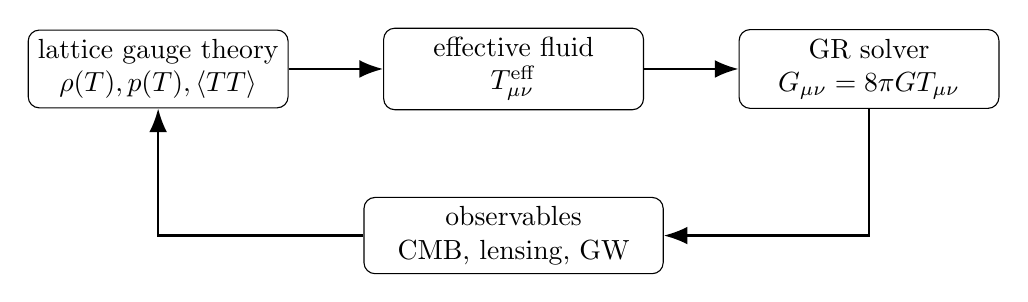
\begin{tikzpicture}[node distance=1.1cm]
    \node[draw,rounded corners,align=center,minimum width=3.3cm] (lat) {lattice gauge theory\\$\rho(T),p(T),\langle TT\rangle$};
    \node[draw,rounded corners,align=center,right=1.2cm of lat,minimum width=3.3cm] (eff) {effective fluid\\$T_{\mu\nu}^{\rm eff}$};
    \node[draw,rounded corners,align=center,right=1.2cm of eff,minimum width=3.3cm] (grav) {GR solver\\$G_{\mu\nu}=8\pi G T_{\mu\nu}$};
    \node[draw,rounded corners,align=center,below=1.1cm of eff,minimum width=3.8cm] (data) {observables\\CMB, lensing, GW};
    \draw[-{Latex[length=3mm]},thick] (lat) -- (eff);
    \draw[-{Latex[length=3mm]},thick] (eff) -- (grav);
    \draw[-{Latex[length=3mm]},thick] (grav) |- (data);
    \draw[-{Latex[length=3mm]},thick] (data) -| (lat);
\end{tikzpicture}
\caption{A realistic workflow uses lattice field theory for matter stress-energy, then separate gravitational evolution.}
\end{figure}


\subsection{Self-consistent semiclassical iteration}
The hybrid algorithm can be promoted from a one-way pipeline to a fixed-point problem. Let $\mathcal L[g]$ denote the lattice map that returns a renormalized matter stress tensor on the prescribed background and let $\mathcal G[T]$ denote the gravitational solver. A self-consistent background satisfies
\begin{equation}
 g_*=(\mathcal G\circ\mathcal L)[g_*].
 \label{eq:lqcd-fixedpoint}
\end{equation}
A practical relaxed iteration is
\begin{equation}
 g_{n+1}=(1-\alpha)g_n+\alpha(\mathcal G\circ\mathcal L)[g_n],
 \qquad 0<\alpha\le1.
 \label{eq:lqcd-relaxation}
\end{equation}
If the linearized map has operator norm
\begin{equation}
 \left\|D(\mathcal G\circ\mathcal L)\big|_{g_*}\right\|<1,
\end{equation}
then the fixed point is locally contractive and the iteration converges for sufficiently close initial data. This gives an explicit numerical criterion for when lattice matter response and classical geometry can be coupled iteratively without promoting the metric to a quantum integration variable.


\section{Where gravitons enter}

In weak-field perturbative quantum gravity, one writes
\begin{equation}
g_{\mu\nu}=\eta_{\mu\nu}+\kappa h_{\mu\nu},
\qquad \kappa^2=32\pi G.
\end{equation}
A graviton is associated with quantized perturbations $h_{\mu\nu}$ after gauge fixing and linearization. A lattice calculation that aims to simulate gravitons must therefore include metric-like degrees of freedom, or a nonperturbative geometry whose fluctuations yield graviton-like correlators in an appropriate continuum limit.

\begin{proposition}[Matter response is not metric dynamics]
The connected stress-energy correlator
\begin{equation}
\langle T_{\mu\nu}(x)T_{\rho\sigma}(y)\rangle_c
\end{equation}
computed in fixed-background QFT is not the graviton propagator. It is a source correlator that may contribute to graviton self-energy or induced-gravity effects in a theory where metric dynamics are added.
\end{proposition}

\begin{proof}[Proof sketch]
A propagator is a two-point function of a dynamical field. In fixed-background QFT, $T_{\mu\nu}$ is an operator built from matter fields, not the metric fluctuation itself. It can source or renormalize gravitational dynamics in an enlarged theory, but it is not identical to $\langle h h\rangle$ without adding a kinetic term and path integral measure for $h_{\mu\nu}$ or geometry.
\end{proof}

\section{Dynamical lattice gravity path}

A quantum-gravity lattice program must replace
\begin{equation}
Z_{\rm matter}[g]
\end{equation}
with something closer to
\begin{equation}
Z=\sum_{\mathcal T} e^{-S_{\rm Regge}[\mathcal T]} Z_{\rm matter}[\mathcal T]
\end{equation}
or an equivalent background-independent measure. In causal dynamical triangulations, one sums over causal triangulated spacetimes with a discrete action related to the Einstein--Hilbert action. Candidate observables include:
\begin{enumerate}[label=(\roman*)]
\item volume profiles;
\item spectral dimension;
\item transfer matrices;
\item curvature-related observables;
\item metric-fluctuation or geometry-correlation proxies.
\end{enumerate}

\section{Computational realism}

Exascale systems can dramatically improve lattice gauge computations, but quantum gravity adds conceptual and algorithmic costs:
\begin{enumerate}[label=(\alph*)]
\item geometry has gauge redundancy/diffeomorphism invariance;
\item observables must be coordinate-independent;
\item Lorentzian path integrals require careful definition or Wick rotation;
\item continuum limits require phase-structure control;
\item adding matter to dynamical geometry increases configuration complexity.
\end{enumerate}

Thus the correct claim is not that current LQCD supercomputers simulate gravitons, but that current and future exascale infrastructure can support pieces of a larger program: lattice stress-energy, hidden-sector equations of state, and lattice-gravity Monte Carlo studies.

\section{Conclusion}

This paper introduced a fixed-background theorem clarifying why standard LQCD cannot directly simulate gravitons. The result is structural: the metric is not in the path-integral measure. The productive path is a tiered program: use lattice gauge theory to compute matter stress-energy, use semiclassical gravity for backreaction, and use dynamical lattice gravity for genuine quantum-geometry questions.

\begin{thebibliography}{99}

\bibitem{Rothe}
H. J. Rothe,
\textit{Lattice Gauge Theories: An Introduction}, World Scientific, 2012.

\bibitem{GattringerLang}
C. Gattringer and C. B. Lang,
\textit{Quantum Chromodynamics on the Lattice}, Springer, 2010.

\bibitem{PDGLattice}
S. Aoki et al.,
``Review of lattice results concerning low-energy particle physics,''
\textit{European Physical Journal C} \textbf{77}, 112 (2017), and updates in Particle Data Group reviews.

\bibitem{YamamotoCurved}
A. Yamamoto,
``Lattice QCD in curved spacetimes,''
\textit{Physical Review D} \textbf{90}, 054510 (2014), arXiv:1405.6665.

\bibitem{LollReview}
R. Loll,
``Quantum gravity from causal dynamical triangulations: a review,''
\textit{Classical and Quantum Gravity} \textbf{37}, 013002 (2020), arXiv:1905.08669.

\bibitem{AmbjornJurkiewiczLoll}
J. Ambj\o rn, J. Jurkiewicz, and R. Loll,
``Dynamically triangulating Lorentzian quantum gravity,''
\textit{Nuclear Physics B} \textbf{610}, 347 (2001), arXiv:hep-th/0105267.

\bibitem{Regge}
T. Regge,
``General relativity without coordinates,''
\textit{Nuovo Cimento} \textbf{19}, 558 (1961).

\bibitem{Donoghue}
J. F. Donoghue,
``General relativity as an effective field theory: the leading quantum corrections,''
\textit{Physical Review D} \textbf{50}, 3874 (1994), arXiv:gr-qc/9405057.

\bibitem{BirrellDavies}
N. D. Birrell and P. C. W. Davies,
\textit{Quantum Fields in Curved Space}, Cambridge University Press, 1982.

\bibitem{WaldQFTCurved}
R. M. Wald,
\textit{Quantum Field Theory in Curved Spacetime and Black Hole Thermodynamics}, University of Chicago Press, 1994.

\end{thebibliography}

\end{document}
